\documentclass[11pt]{article}

\usepackage{amssymb}
\usepackage{xcolor}
\usepackage{verbatim}
\usepackage{multicol}
\usepackage{enumitem}
\usepackage{amsfonts}
\usepackage{amsmath}
\usepackage[utf8]{inputenc}
\usepackage[export]{adjustbox}  % for correct logo rendering
\usepackage{fancyhdr}  % for header/footer formatting
\usepackage{hyperref}  % for hyper-references
\usepackage{datetime}  % to update month in footer
\usepackage{array}  % more flexible tables
\usepackage[includeheadfoot,
            left=1in,
            right=1in,
            top=0.75in,
            bottom=0.75in,
            headheight=40pt]{geometry} % geometry needs to know headheight to correctly render the footer
\usepackage{tikz} % For drawing grid boxes

\definecolor{darkblue}{RGB}{0, 0, 139}
\definecolor{lightblue}{RGB}{173, 216, 230}

% desired format for footer
\newdateformat{monthyeardate}{%
  \monthname[\THEMONTH] \THEYEAR}

% set up header/footer
\pagestyle{fancy}
\fancyhf{}  % clear all headers/footers
\renewcommand{\headrulewidth}{0pt}  % remove header rule
\renewcommand{\footrulewidth}{0pt}  % remove footer rule

% set up header

\fancypagestyle{firstpage}{
    \fancyhead[L]{
    \vspace{0pt}
    \hspace{-8pt}
    
\includegraphics[width=0.1\textwidth]{docimgs/eth_logo_kurz_pos.png}\\
    \textbf{Swiss Federal Institute of Technology}\\
    \textbf{Zurich}\\
    %\textbf{ } \\
    
    }    

    \fancyhead[R]{
    \raggedleft
    %\vspace{20pt}
    
\includegraphics[width=0.13\textwidth]{docimgs/eth_ditet_logo_pos.png}\\
     \textbf{Dept. of Information Technology and} \\ \textbf{Electrical Engineering}  \\
     %\textbf{Chair for Mathematical Information} \\ \textbf{Information Science} \\

    }
}

% set up footer
\fancyfoot[L]{mdietz, ÜS 3}
\fancyfoot[C]{\thepage}
\fancyfoot[R]{\monthyeardate\today}

% set up section/subsection titles
\renewcommand{\thesection}{\arabic{section}}
\renewcommand{\thesubsection}{\arabic{subsection}}

% command used for simply emphasizing suggestions
\newcommand{\suggestion}[1]{{\itshape #1}}


\begin{document}
\thispagestyle{firstpage}

\setlength{\headheight}{1 \baselineskip}  % accomodate header
\setlength{\parindent}{0pt}  % remove initial paragraph indent
\setlength{\parskip}{\baselineskip}  % add skip between paragraphs

\vspace*{-5px}
\section*{Übungsstunde 3}

\section*{Themenüberblick}
\begin{itemize}
    \item \textbf{Systeme und Systemeigenschaften:}
    \item[] Linearität, Nullraum und Bildraum, Stetigkeit
    \item[] Das inverse System
    \item[] Darstellung linearer Systeme über Matrizen
    \item \textbf{Eigenschaften zeitkontinuierlicher linearer Systeme}
    \item[] Zeitinvarianz, Kausalität, Gedächtnis, BIBO-Stabilität
\end{itemize}

\section*{Aufgaben für diese Woche}
\vspace{-0.5cm}

25, 26, \underline{\textbf{27}}, \underline{\textbf{28}}, \underline{\textbf{29}}, 30, \underline{\textbf{32}}\\
\vspace{-0.5cm}

Die \underline{\textbf{fettgedruckten}} Übungen empfehle ich, weil sie wesentlich zu eurem Verständnis der Theorie beitragen und/oder sehr prüfungsrelevant sind.

\vfill \null
\pagebreak

\section*{Systeme und Systemeigenschaften}
\vspace*{-0.5cm}
\hspace{-0.3cm}
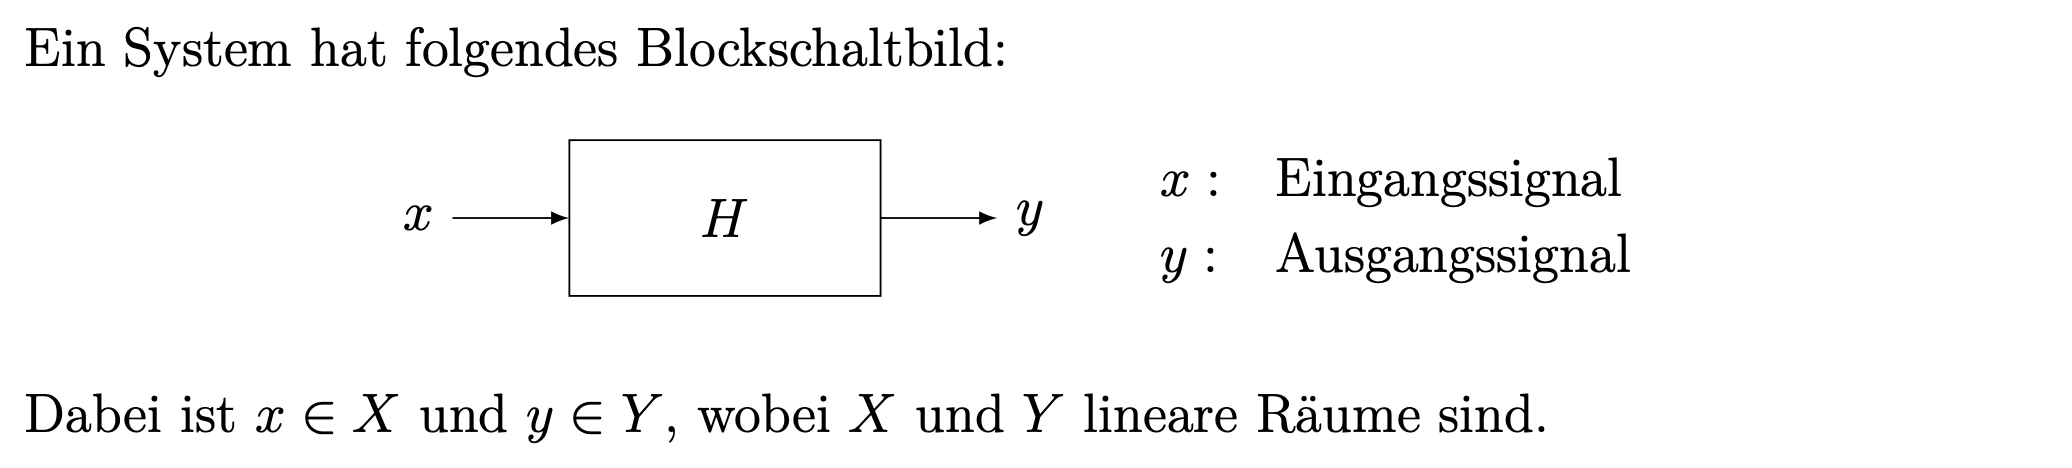
\includegraphics[width=0.95\linewidth]{docimgs/System_Blockschaltbild.png}

\textbf{Definition:} Ein System $H$ ist eine Abbildung, die einem Eingangssignal $x$ ein Ausgangssignal $y$ zuordnet. Man schreibt $y = Hx$

\subsection*{Linearität}
\vspace*{-0.5cm}
\textbf{Definition:} Ein System $H:X \to Y$ ist linear, wenn 
\vspace*{-0.5cm}
\begin{itemize}
    \item[(i)] Additivität: $H(x_1 + x_2) = Hx_1 + Hx_2$, für alle $x_1,x_2 \in X$
    \item[(ii)] Homogenität: $H(\alpha x) = \alpha H x$, für alle $x\in X$ und alle $\alpha \in \mathbb{C}$
\end{itemize}
\textbf{Bemerkungen:}
\vspace*{-0.5cm}
\begin{itemize}
    \item Ein System, das mindestens eine dieser beiden Bedingungen nicht erfüllt, heisst \textbf{nichtlinear}.
    \item Wenn $H$ ein lineares System ist, dann muss immer gelten: $H0 = 0$. Wenn dies also nicht erfüllt ist, dann muss $H$ nichtlinear sein.
\end{itemize}

\vfill \null
\pagebreak

\subsection*{Nullraum}
\vspace*{-0.5cm}
\begin{itemize}[leftmargin = 0pt]
    \item[] \textbf{Definition:} Der Nullraum $\mathcal{N}(H)$ des linearen Systems $H:X \to Y$ ist die Teilmenge von $X$ definiert durch $\mathcal{N}(H) = \{x \in X : Hx = 0\}$.
    \item[] \textbf{Bemerkung:} $\mathcal{N}(H)$ ist ein linearer Unterraum von $X$.
\end{itemize}

\subsection*{Bildraum}
\vspace*{-0.5cm}
\begin{itemize}[leftmargin = 0pt]
    \item[] \textbf{Definition:} Der Bildraum $\mathcal{R}(H)$ des linearen Systems $H:X \to Y$ ist die Teilmenge von $Y$ definiert durch $\mathcal{R}(H) = \{y =Hx : x \in X\}$.
    \item[] \textbf{Bemerkung:} $\mathcal{R}(H)$ ist ein linearer Unterraum von $Y$.
\end{itemize}

\begin{center}
    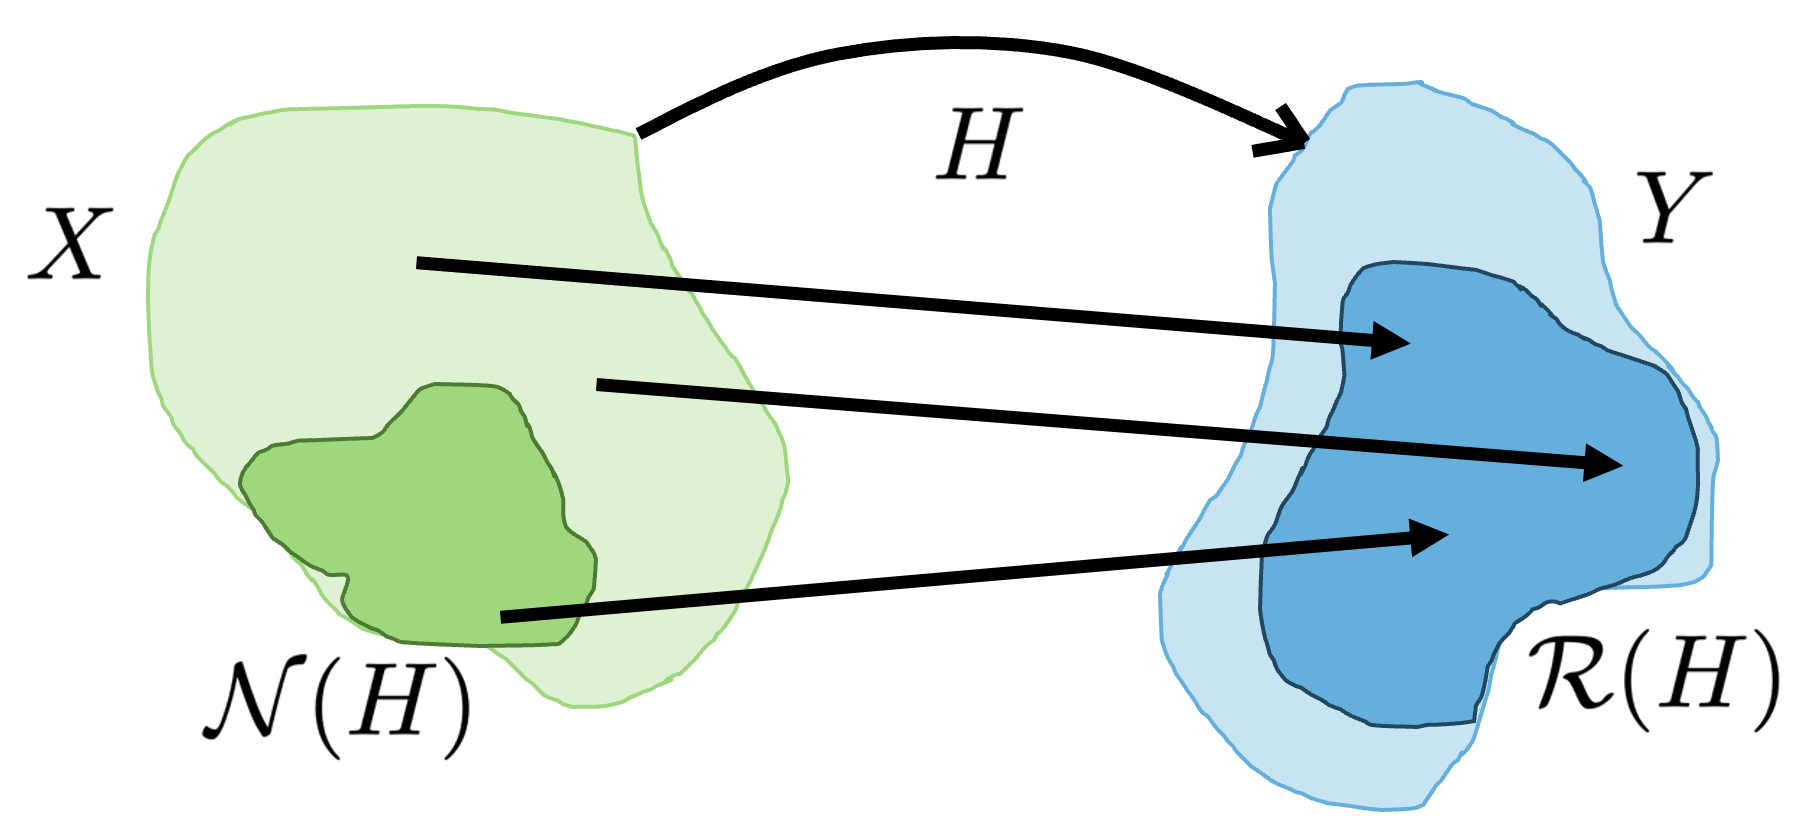
\includegraphics[width = 0.7\linewidth]{docimgs/Bildraum_Nullraum.png}
\end{center}


\subsection*{Stetigkeit}
\vspace*{-0.5cm}
\begin{itemize}[leftmargin = 0pt]
    \item[] \textbf{Theorem:} (\textit{Stetige Systeme}). Das System $H$ ist linear und stetig, dann und nur dann, wenn für jede konvergente Reihe $\sum_{i=1}^\infty \alpha_i x_i$ gilt:
    $$H\left( \sum_{i=1}^\infty \alpha_i x_i \right) = \sum_{i=1}^\infty \alpha_i H x_i$$
    \item[] \textbf{$\varepsilon-\delta$ Stetigkeit} (vgl. Analysis $1 \& 2$).\\Seien $(X, ||\cdot||)$ und $(Y, ||\cdot||)$ normierte lineare Räume. Dann heisst das System $H:X \to Y$ stetig in $x_0 \in X$, falls es zu jedem $\varepsilon > 0$ ein nur von $\varepsilon$ abhängiges $\delta >0$ gibt, so dass für alle $x\in X$ mit $||x-x_0||<\delta$ folgt, dass $||Hx-Hx_0||\leq \varepsilon$.
    \item[] \textbf{Bemerkung:} Ab hier nehmen wir in SST1 immer an, dass ein lineares Sysem auch stetig ist, sodass die Gleichung in obigem Theorem immer gilt.
\end{itemize}

\vfill \null
\pagebreak

\subsection*{Das inverse System}
\vspace*{-0.5cm}
\begin{itemize}[leftmargin=0pt]
    \item[] Das System $H:X \to Y$ ist \textbf{invertierbar}, wenn es ein System $G:Y \to X$ gibt, so dass $GH = I_X$ und $HG = I_Y$, wobei $I_X$ bzw. $I_Y$ die Identitätsabbildungen auf $X$ bzw. $Y$ sind. (D.h. $I_X x = x$, für alle $x\in X$ und $I_Y y= y$, für alle $y \in Y$.) In diesem Fall bezeichnen wir $G$ als das zu $H$ zugehörige inverse System und schreiben $H^{-1} = G$.
    \item[] Wenn ein System invertierbar ist, dann ist seine Inverse \textbf{eindeutig}.
    \item[] \textbf{Beweis}:
    \item[] 
\begin{tikzpicture}
    % Define the box size and grid spacing
    \draw[step=0.5cm,gray!50,very thin] (0,0) grid (16.5,3); % (0,0) is bottom-left corner, (10,10) is top-right corner
\end{tikzpicture}
    \item[] \textbf{Theorem}: Die Inverse eines linearen Systems ist auch linear.
    \item[] \textbf{Beweis}:
    \item[] 
\begin{tikzpicture}
    % Define the box size and grid spaci
    \draw[step=0.5cm,gray!50,very thin] (0,0) grid (16.5,5); % (0,0) is bottom-left corner, (10,10) is top-right corner
\end{tikzpicture}
\end{itemize}

\vfill \null
\pagebreak

\subsection*{Darstellung linearer Systeme über Matrizen}
\vspace*{-0.5cm}
Man kann ein allgemeines endlich-dimensionales lineares System $H$ durch eine Matrix beschreiben. Dazu betrachten wir die linearen Räume $X$ und $Y$ mit den zugehörigen Basen $B_1 = \{x_1, \dots, x_n\}$ und $B_2 = \{ y_1, \dots, y_m \}$. $x\in X$ ist das Eingangssignal und $y=Hx \in Y$ das dazugehörige Ausgangssignal. Jedes $x\in X$ und jedes $y\in Y$ lässt sich wie folgt darstellen:
$$x = \alpha_1 x_1 + \dots + \alpha_n x_n, \hspace{12pt} \text{wobei } \{\alpha_1, \dots, \alpha_n\} \text{ die Koffizienten von } x \text{ sind.}$$
$$y = \beta_1 y_1 + \dots + \beta_m y_m, \hspace{12pt} \text{wobei } \{\beta_1, \dots, \beta_m\} \text{ die Koffizienten von } y \text{ sind.}$$
$$\text{Wir wenden }H \text{ auf } x \text{ an:} \hspace{24pt} Hx = H(\alpha_1 x_1 + \dots + \alpha_n x_n) = \alpha_1 Hx_1 + \dots + \alpha_n Hx_n, \hspace{40pt} \text{(Lin.)}$$
Da $Hx_1, \dots, Hx_n$ in $Y$ sind, können wir sie wie folgt darstellen:
\begin{align*}
    Hx_1 &= t_{11}y_1 + \dots + t_{m1}y_m \\
    Hx_2 &= t_{12}y_1 + \dots + t_{m2}y_m \\
    &\hspace{6pt}\vdots \\
    Hx_n &= t_{1n}y_1 + \dots + t_{mn}y_m
\end{align*}
\begin{align*}
    \implies Hx &= \alpha_1(t_{11}y_1 + t_{21}y_2 + \dots + t_{m1}y_m) \\
    &\hspace{1pt}+ \alpha_2(t_{12}y_1 + t_{22}y_2 + \dots + t_{m2}y_m) \\
    &\hspace{6pt}\vdots \\
    &\hspace{1pt}+ \alpha_n(t_{1n}y_1 + t_{2n}y_2 + \dots + t_{mn}y_m) \\
    &= \overbrace{(t_{11}\alpha_1 + t_{12}\alpha_2 + \dots + t_{1n}\alpha_n)}^{\beta_1}y_1 \\
    &\hspace{1pt}+ \smash{\underbrace{(t_{21}\alpha_1 + t_{22}\alpha_2 + \dots + t_{2n}\alpha_n)}_{\beta_2}}y_2\\
    &\hspace{6pt}\vdots \\
    &\hspace{1pt}+ \underbrace{(t_{m1}\alpha_1 + t_{m2}\alpha_2 + \dots + t_{mn}\alpha_n)}_{\beta_m}y_m
\end{align*}
In Matrixform sieht das Ganze wie folgt aus:
$$\begin{bmatrix}
    \beta_1 \\ \beta_2 \\ \vdots \\ \beta_m
\end{bmatrix} = \underbrace{\begin{bmatrix}
    t_{11} & t_{12} & \dots & t_{1n} \\
    t_{21} & t_{22} & \dots & t_{2n} \\
    \vdots & \vdots & \ddots & \vdots \\
    t_{m1} & t_{m2} & \dots & t_{mn} \\
\end{bmatrix}}_{\mathbf{H}} \cdot \begin{bmatrix}
    \alpha_1 \\ \alpha_2 \\ \vdots \\ \alpha_n
\end{bmatrix}$$
Man sagt, dass die $m \times n$ Matrix $\mathbf{H}$ das System $H$ in den Basen $B_1$ und $B_2$ darstellt.

\vfill \null
\pagebreak

\subsection*{Aufgabe 25}
\vspace*{-0.5cm}
Seien $X$ und $Y$ die linearen Räume aller Polynome vom Grad $\leq 3$ bzw. $\leq 2$:
$$X = \{ x(t) = \alpha_0 + \alpha_1 t + \alpha_2 t^2 + \alpha_3 t^3 \; | \; \alpha_i \in \mathbb{C} \}, \hspace{40pt} Y = \{ y(t) = \beta_0 + \beta_1 t + \beta_2 t^2 \; | \; \beta_j \in \mathbb{C} \}$$
Wir definieren das System $H:X \to Y$ mit $Hx = \frac{\text{d}x(t)}{\text{d}t}$ (Ableitungsoperator).
\vspace*{-0.5cm}
\begin{itemize}
    \item[a)] Zeigen Sie, dass $H$ linear ist und $\mathcal{R}(H) = Y$.
    \item[b)] Berechnen Sie für die Basis $B_1 = \{1, t, t^2, t^3\}$ von $X$ und die Basis $B_2 = \{ 1, t, t^2 \}$ von $Y$ die Matrixdarstellung von $H$.
\end{itemize}
\vspace*{-0.5cm}

\begin{tikzpicture}
    % Define the box size and grid spacing
    \draw[step=0.5cm,gray!50,very thin] (0,0) grid (16.5,16); % (0,0) is bottom-left corner, (10,10) is top-right corner
\end{tikzpicture}

\pagebreak

\subsection*{Aufgabe 26}
\vspace*{-0.5cm}
Seien $X$ und $Y$ die linearen Räume aller Polynome vom Grad $\leq 3$ bzw. $\leq 2$:
$$X = \{ x(t) = \alpha_0 + \alpha_1 t + \alpha_2 t^2 + \alpha_3 t^3 \; | \; \alpha_i \in \mathbb{C} \}, \hspace{40pt} Y = \{ y(t) = \beta_0 + \beta_1 t + \beta_2 t^2 \; | \; \beta_j \in \mathbb{C} \}$$
Wir definieren das System $H:X \to Y$ mit $Hx = \frac{\text{d}x(t)}{\text{d}t}$ (Ableitungsoperator). Berechnen Sie die Matrixdarstellung von $H$ unter Verwendung der Basen $B_1 = \{ 1 + t, t + t^2, t^2 + t^3, t^3 \}$ für $X$ und $B_2 = \{ 1, t, t^2 \}$ für $Y$.\\

\vspace{-0.65cm}

\begin{tikzpicture}
    % Define the box size and grid spacing
    \draw[step=0.5cm,gray!50,very thin] (0,0) grid (16.5,17); % (0,0) is bottom-left corner, (10,10) is top-right corner
\end{tikzpicture}

\pagebreak

\section*{Eigenschaften zeitkontinuierlicher linearer Systeme}

\vspace*{-0.5cm}
\subsection*{Zeitinvarianz}
\vspace*{-0.5cm}
\begin{itemize}[leftmargin=0pt]
    \item[] \textbf{Definition}: Ein System $H:X \to Y$ ist \textbf{zeitinvariant}, wenn
    $$HT_\tau x = T_\tau Hx, \text{ für alle } x \in X, \; \tau \in \mathbb{R}$$
    \item[] $(T_\tau x)(t) := x(t-\tau)$ ist der Zeitverschiebungsoperator. Ein System, das nicht zeitinvariant ist, heisst \textbf{zeitvariant}.
    \item[] \textbf{Intuition}: Zeitverschiebung am Eingang des Systems führt zu derselben Zeitverschiebung am Ausgang des Systems.
\end{itemize}

\subsection*{Kausalität}
\vspace*{-0.5cm}
\begin{itemize}[leftmargin=0pt]
    \item[] \textbf{Definition}: Ein System $H:X \to Y$ ist \textbf{kausal}, wenn für alle $x_1, x_2 \in X$ und jedes $T\in \mathbb{R}$ gilt
    $$x_1(t) = x_2(t), \hspace{10pt} \text{für alle } t \leq T \implies (Hx_1)(t) = (Hx_2)(t), \hspace{10pt} \text{für alle } t \leq T.$$
    \item[] \begin{center}
        \vspace*{-0.5cm}
        \includegraphics[width=0.8\linewidth]{docimgs/Kausalität.png}
    \end{center}
    \item[] \textbf{Intuition}: Das Ausgangssignal zu dem Zeitpunkt $T$ kann nur von dem momentanen oder den vergangenen Zeitpunkten abhängig sein. Der Ausgang des Systems ist nicht von zukünftigen Werten abhängig.
    \item[] Echtzeitrealisierungen sind immer kausal.
\end{itemize}

\subsection*{Gedächtnis}
\vspace*{-0.5cm}
\begin{itemize}[leftmargin=0pt]
    \item[] \textbf{Definition}: Ein System $H:X \to Y$ ist \textbf{gedächtnislos}, wenn für alle $x\in X$ und alle Zeitpunkte $t_0 \in \mathbb{R}$ das Ausgangssignal $(Hx)(t)$ zum Zeitpunkt $t_0$, d.h., $(Hx)(t_0)$, nur von $x(t_0)$ abhängt. Erfüllt ein System diese Eigenschaft nicht, dann bezeichnen wir es als \textbf{gedächtnisbehaftet}.
    \item[] Gedächtnislosigkeit $\implies$ Kausalität aber nicht umgekehrt.
\end{itemize}

\vfill \null
\pagebreak

\subsection*{BIBO-Stabilität}
\vspace*{-0.5cm}
\begin{itemize}[leftmargin=0pt]
    \item[] \textbf{Definition}: Ein System $H:X\to Y$ ist \textbf{BIBO-stabil} (\textit{bounded input bounded output stabil}), wenn für alle $x\in X$ mit $|x(t)| \leq B_x < \infty$, für alle $t$, ein $B_y \in \mathbb{R}$ mit $B_y < \infty$ existiert, sodass $|y(t)| \leq B_y$, für alle $t$, wobei $y=Hx$.
    \item[] \textbf{Intuition}: Jedes beschränkte Eingangssignal führt zu einem beschränkten Ausgangssignal. 
\end{itemize}

\subsection*{Aufgabe 28}
\vspace*{-0.5cm}
Überprüfen Sie das System
$(Hx)(t) = tx(t),$
auf Zeitinvarianz.

\vspace*{-0.2cm}

\begin{tikzpicture}
    % Define the box size and grid spacing
    \draw[step=0.5cm,gray!50,very thin] (0,0) grid (16.5,6); % (0,0) is bottom-left corner, (10,10) is top-right corner
\end{tikzpicture}

\subsection*{Prüfungsaufgabe: Frühjahr 2024, Aufgabe 1.a)i. (1 Punkt)}
\vspace*{-0.5cm}
Ist das System $H_3$ mit Eingangs-Ausgangsbeziehung $(H_3 x)(t) = \frac{dx(t)}{dt}$ ein LTI-System? \\
\textit{Hinweis: Sie können die Stetigkeit des Operators $\frac{dx(t)}{dt}$ ohne Beweis annehmen.}

\vspace*{-0.25cm}

\begin{tikzpicture}
    % Define the box size and grid spacing
    \draw[step=0.5cm,gray!50,very thin] (0,0) grid (16.5,6); % (0,0) is bottom-left corner, (10,10) is top-right corner
\end{tikzpicture}

\pagebreak

\subsection*{Aufgabe 29}
\vspace*{-0.5cm}
Überprüfen Sie die folgenden Systeme auf Kausalität und BIBO-Stabilität.
\begin{multicols}{2}
    \begin{itemize}
        \item[a)] $(Hx)(t) = \displaystyle \frac{1}{2}(x(t-1) + x(t+1))$
        \item[b)] $(Hx)(t) = \displaystyle \int_{t-2}^{t-1} x(\tau + 1)d\tau$
    \end{itemize}
\end{multicols}

\vspace*{-0.5cm}
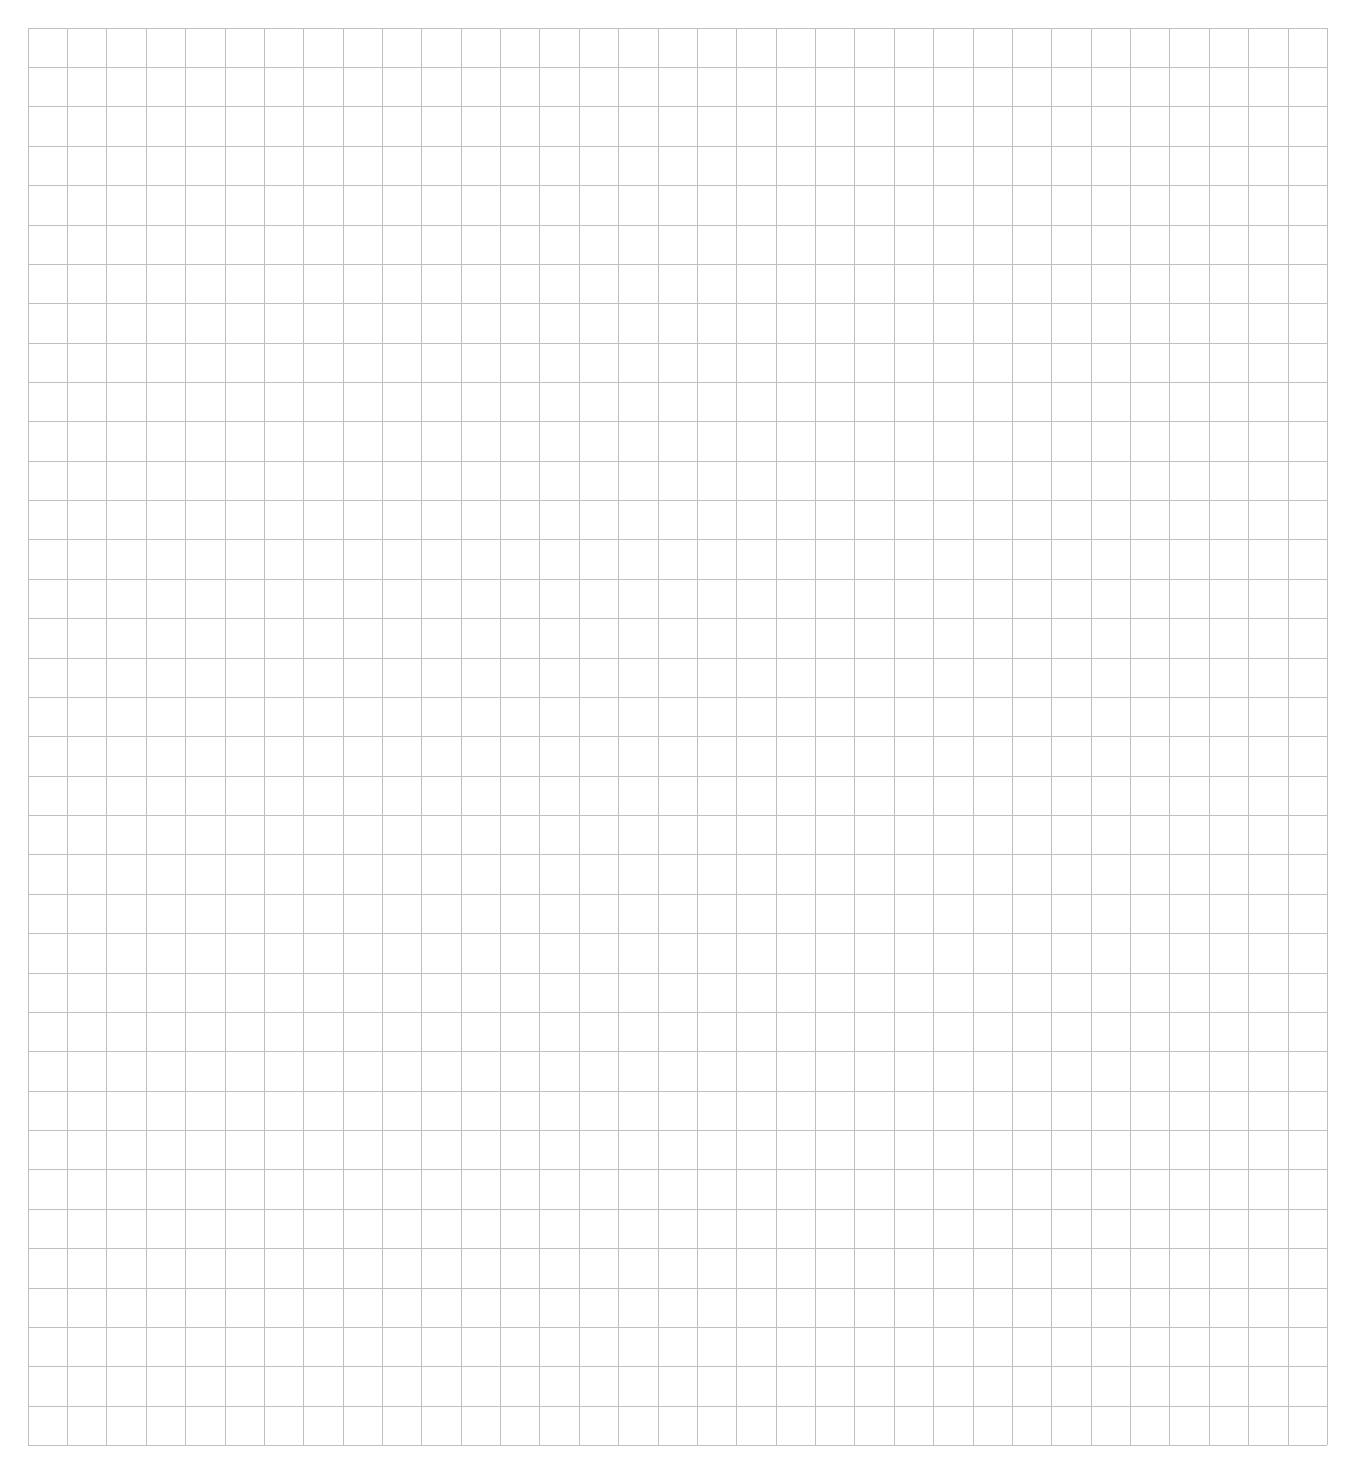
\begin{tikzpicture}
    % Define the box size and grid spacing
    \draw[step=0.5cm,gray!50,very thin] (0,0) grid (16.5,18); % (0,0) is bottom-left corner, (10,10) is top-right corner
\end{tikzpicture}

\end{document}